\subsection{Network coherence audit: STRING edges in CLIP target sets are explained by expression (negative)}
The g:Profiler section tests term enrichment; STRING v12.0 tests whether a target set is more densely connected than chance (\texttt{scripts/string\_coherence.py}; \texttt{results/string\_coherence.json}; hermetic tests). Same panel, sets and seeds as above; the statistic is the edge density $\rho=E/\binom{n}{2}$ among mapped query proteins with STRING combined score $\geq 0.7$. Gates passed: the cell-cycle control gives 133 edges (bar 50); median random density 0.00145 (bar 0.01); median mapped fraction 97.5\%.
CNN top-200 sets are no denser than random (H1: 6 wins, 7 losses, $p=0.709$, falsified) and lose to the expression top-200 control on 13/13 (H3, falsified). CLIP-positive sets are denser than random on 13/13 ($p=1.2\times10^{-4}$), so pre-registered H2 is confirmed. Because CLIP detection depends on expression, we then added a post-hoc control that we did not pre-register: random sets drawn from each miRNA's universe to match the CLIP set's HEK293 expression-decile histogram. Against it the CLIP excess does not survive (8 wins, 4 losses, one tie excluded, $p=0.194$; Figure~\ref{fig:string}).
So the one positive in this audit is explained by expression, the same confound that dominates the CLIP labels and the g:Profiler terms. We report H2 as confirmed-then-explained, not as evidence that miRNA targets form network modules.
\begin{figure}[h]\centering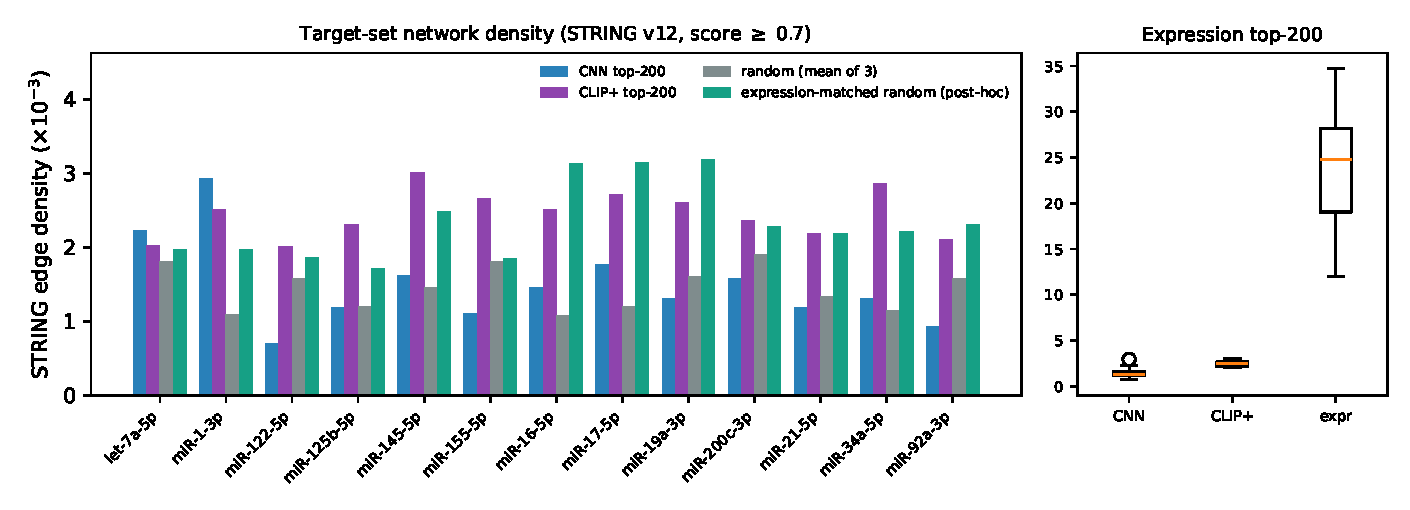
\includegraphics[width=0.95\linewidth]{figs/fig_string.pdf}
\caption{Left: STRING edge density per miRNA for CNN top-200, CLIP+ top-200, seeded random and expression-matched random sets. Right: distribution across miRNAs with the expression top-200 control, which is several-fold denser.}\label{fig:string}\end{figure}
